\par{Listing \ref{tiling} the last optimisation for matrix multiplication. In
    this \emph{kernel} we pass from host code 2 arrays allocated in \emph{local
    memory} to store tiles of matrix A and B. This \emph{kernel} is executed in
    phases enforced by barrier synchronization inside of every \emph{work group}.
    The code shows in listing \ref{tiling} shows that every \emph{work item} loads
    2 elements for the tile(one from A and one from B), these elements are reused 
    by different \emph{work items} in the \emph{work group}, all \emph{work items
    } in a \emph{work group} calculate part of the block of the resulting matrix.}

\par{The results of this \emph{kernel} are shown in figure \ref{tilingResults},
    this \emph{kernel} shows the best L1 cache hit ratio of all the \emph{
        kernels} exercised in this report.}

\begin{figure}[!h]
    \centering
    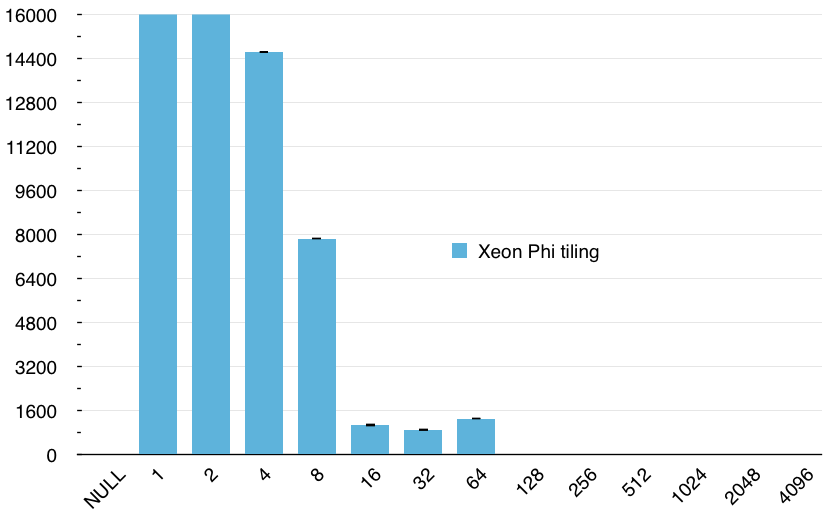
\includegraphics[width=0.4\textwidth]{figures/phiTiling.png}
    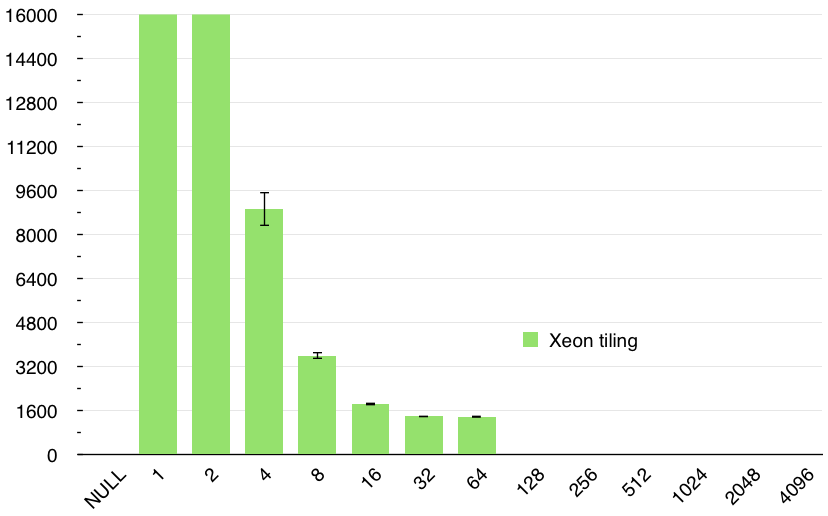
\includegraphics[width=0.4\textwidth]{figures/xeonTiling.png}
    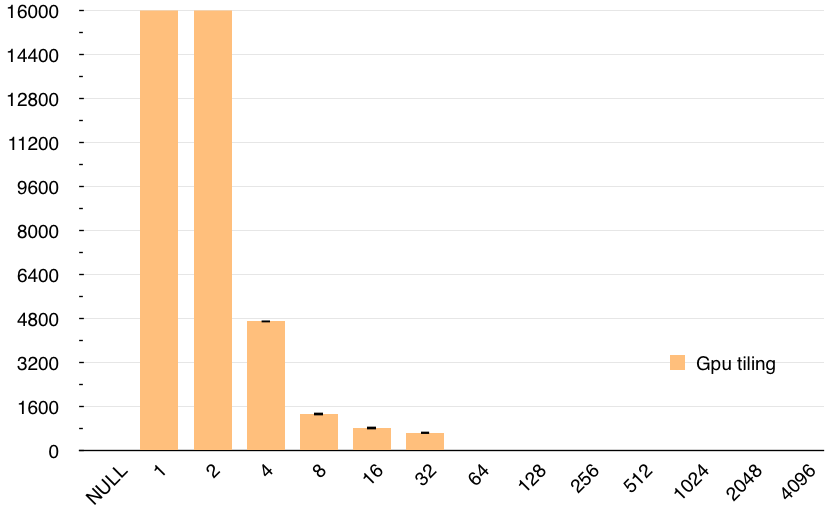
\includegraphics[width=0.4\textwidth]{figures/gpuTiling.png}
    \caption{Results for tiling.}
    \label{tilingResults}
\end{figure}

\par{Figure \ref{gpu}, \ref{phi} and \ref{xeon} show that this optimisation 
    results in the best execution time in comparison against all the other
    \emph{kernels}.}

\subsubsection{Summary Matrix Matrix Multiplication}

\par{Figure \ref{gpu}, \ref{phi} and \ref{xeon} shows the summary of the results of all the changes in the kernels for matrix
    matrix multiplication.}

\begin{figure}[!h]
    \centering
    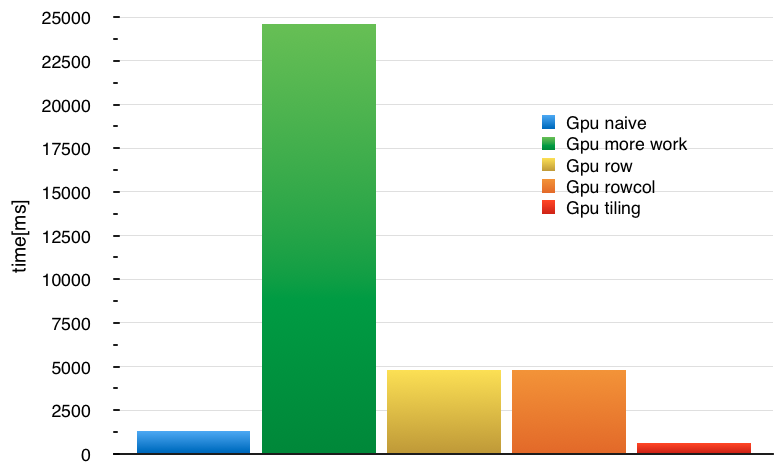
\includegraphics[width=0.4\textwidth]{figures/gpu.png}
    \caption{Matrix Matrix multiplication optimisations GPU.}
    \label{gpu}
\end{figure}

\begin{figure}[!h]
    \centering
    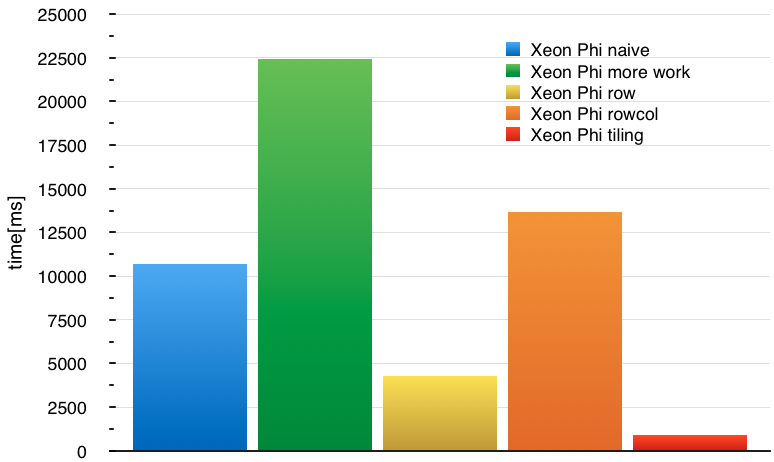
\includegraphics[width=0.4\textwidth]{figures/phi.png}
    \caption{Matrix Matrix multiplication optimisations Xeon Phi.}
    \label{phi}
\end{figure}

\begin{figure}[!h]
    \centering
    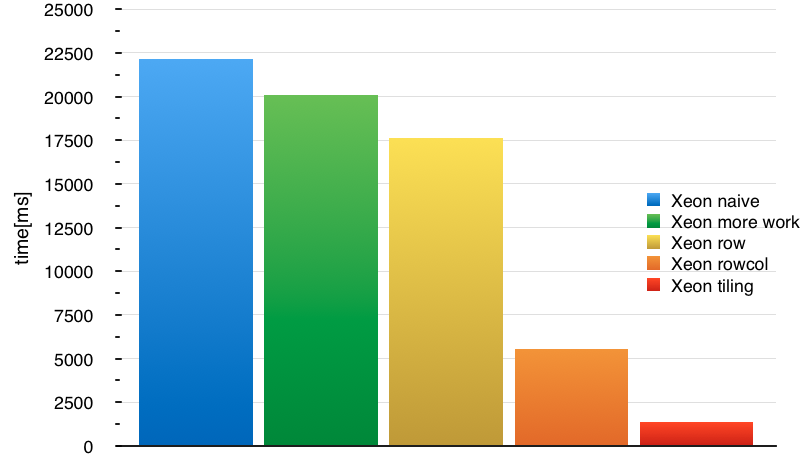
\includegraphics[width=0.4\textwidth]{figures/xeon.png}
    \caption{Matrix Matrix multiplication optimisations Xeon.}
    \label{xeon}
\end{figure}

